\documentclass[a4paper,kulak]{kulakarticle}

\usepackage[utf8]{inputenc}
\usepackage[dutch]{babel}
\usepackage{pdfpages}


\date{\today}
\address{
	Bachelor in de fysica\\
	Bachelor in de informatica\\
	Bachelor in de wiskunde\\
	Ingenieurswetenschappen}
\title{BDA App}
\author{Marthe B\"{o}ting\\
	Robin Bruneel\\
	Toon Ingelaere}

\begin{document}
	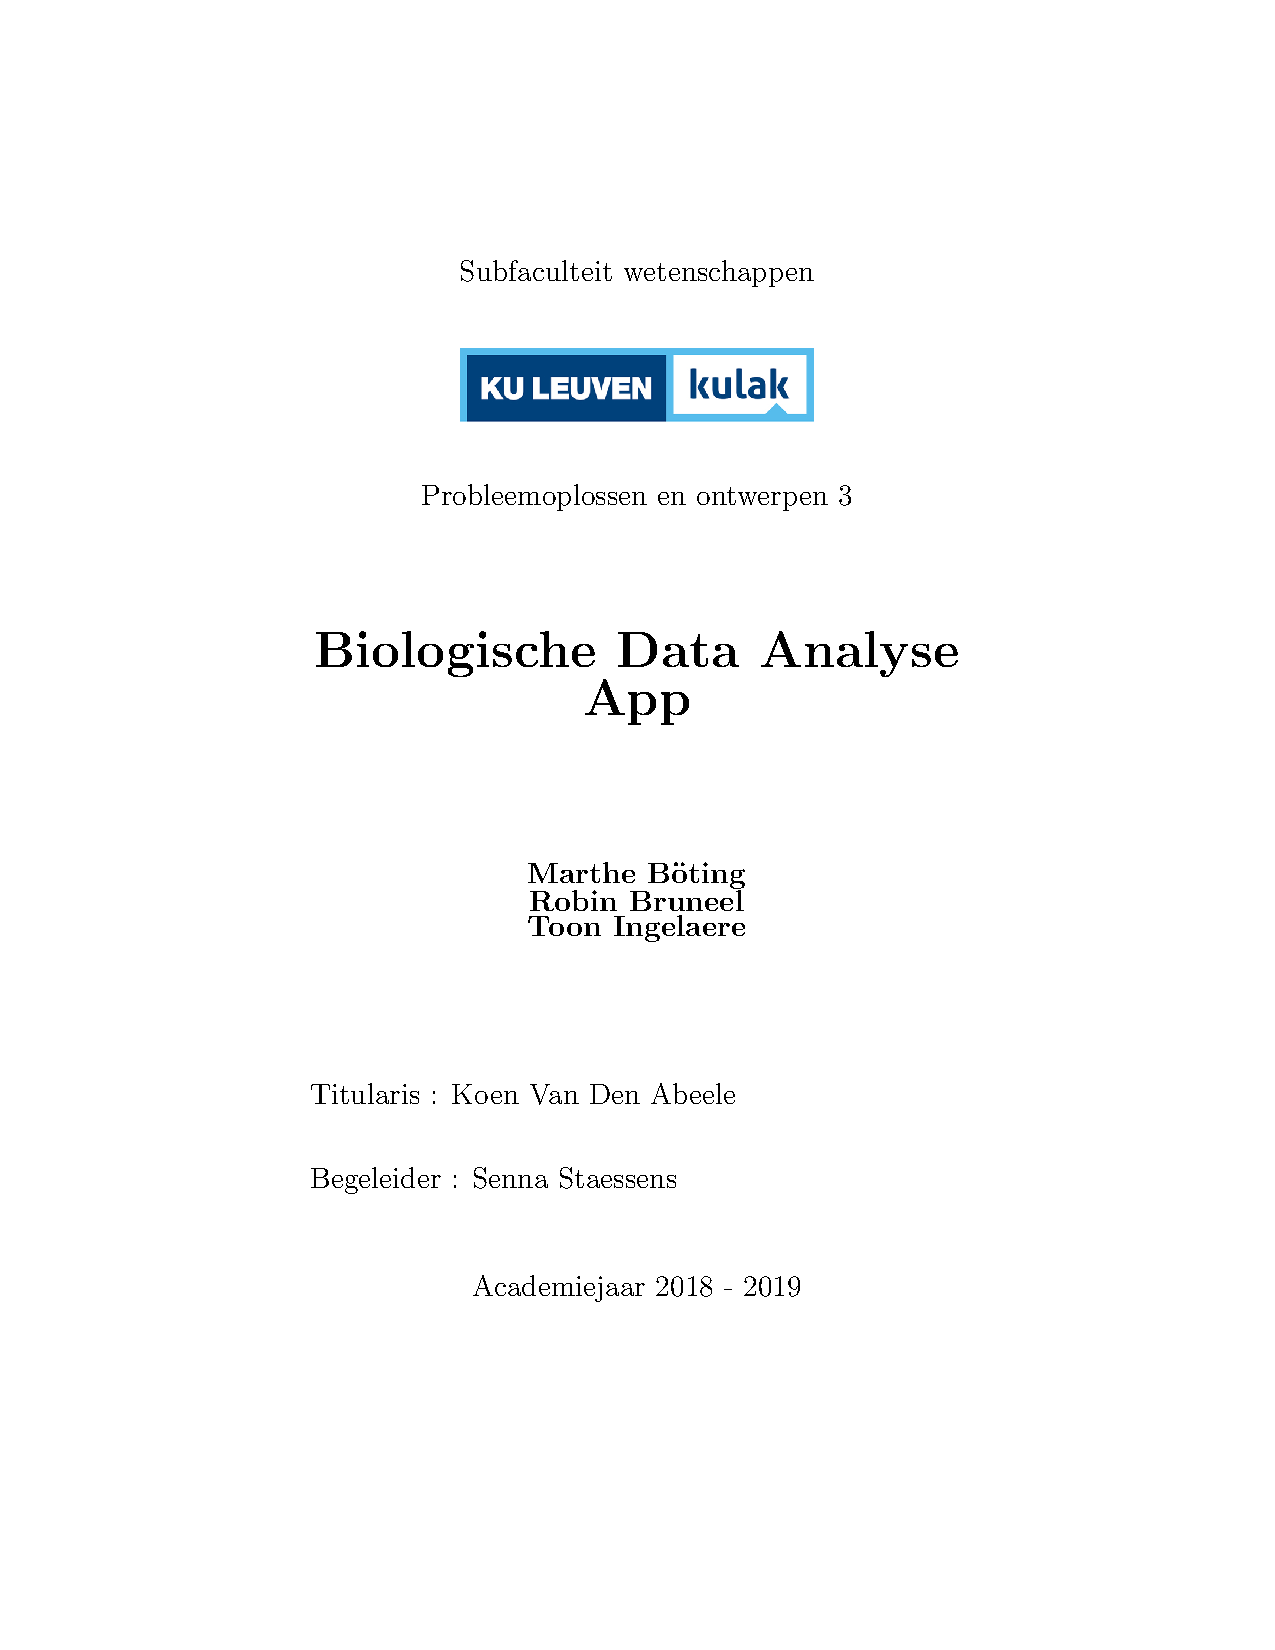
\includepdf{voorblad}
	\newpage
	\maketitle
	\tableofcontents
	\newpage
	
	\section*{Inleiding}	
		Als gevolg van een bloedklonter in een hersenbloedvat ontstaat een ischemische beroerte. Deze klonter moet men zo snel mogelijk verwijderen dit kan met behulp van een geneesmiddel die de klonter oplost of door middel van mechanische verwijdering. Door deze mechanische verwijdering kan men de bloedklonter verder analyseren in het labo om een duidelijker beeld te krijgen.
		\newline
		Vandaag de dag verliest men zeer veel tijd aan het verwerken van de bloedklonters. Er is ons dan ook gevraagd om een app te ontwikkelen die de analyse van de foto’s volledig automatisch kan uitvoeren.
		\newline
		In dit verslag gaan we eerst in op wat de klant specifiek van ons verwacht en aan welke specificaties ons ontwerp moet voldoen. Hierna gaan we ons design bespreken en toelichten. Verder bespreken we ook onze voorlopige resultaten. Ten slotte wordt er nog een blik geworpen naar de vakken uit eerste 3 semesters die ons hierbij geholpen hebben.
	
	\section{Klantenvereisten}
		De klant verwacht een gebruiksvriendelijke app waarbij hij een foto kan ingeven en dat deze automatisch bewerkt wordt. De foto moet  worden bijgesneden en de achtergrond moet verwijderd worden. Daarnaast is het de bedoeling om de bloedklonter te analyseren met andere woorden het berekenen van het percentage van een eiwit. Dit gebeurt door een hoeveelheid kleur te quantificeren in de bloedklonter. 
	
	\section{Ontwerpspecificatie}
		De klant wil een app die elke foto kan bijwerken en ook een percentage van de eiwitten weergeven. Er zijn geen verdere voorwaarden verbonden aan de grootte van de foto. Een absolute voorwaarde om de foto bij te snijden is dat de bloedklonter er volledig opstaat. Desondanks mag de rand niet te groot zijn omdat dit anders te veel geheugen in beslag neemt. De achtergrond moet volledig wit gemaakt worden zodat er geen fouten worden gemaakt bij het berekenen van een hoeveelheid kleur. De app moet voor iedereen bruikbaar zijn. Daarnaast moeten de verschillende foto's over de verschillende fasen getoond worden.
		
	\section{Oplossing} 

		\subsection{App}
		Momenteel zijn dit nog afzonderlijke programma's waarbij we steeds zelf de te aan te passen foto erin inzetten. Naar de klant toe is dit geen manier van werken en wordt dit in een app samengebracht. De klant zal dan zelf kunnen ingeven welke foto hij wil laten verwerken. Eénmaal de foto gekozen is , zal in de eerste fase de achtergrond van de foto wit worden gemaakt en zal de foto afgesneden worden zodanig dat enkel de bloedklonter zichtbaar is. Als dit gebeurd is , zal er al een eerste resultaat getoond worden. Hierdoor heeft de klant een beeld waarop de verdere analyse zal gebeuren en kan die eventueel ingrijpen bij fouten. Vervolgens zal de kleurenanalyse gebeuren. Ook hiervoor zal de foto getoond worden waarop de klant kan zien welke delen de indicator bevatten en zal het percentage gegeven worden. De basis van de app hebben we al zoals te zien is in onderstaande figuur \ref{fig: app}
	
		\begin{figure}[H]
			\centering
			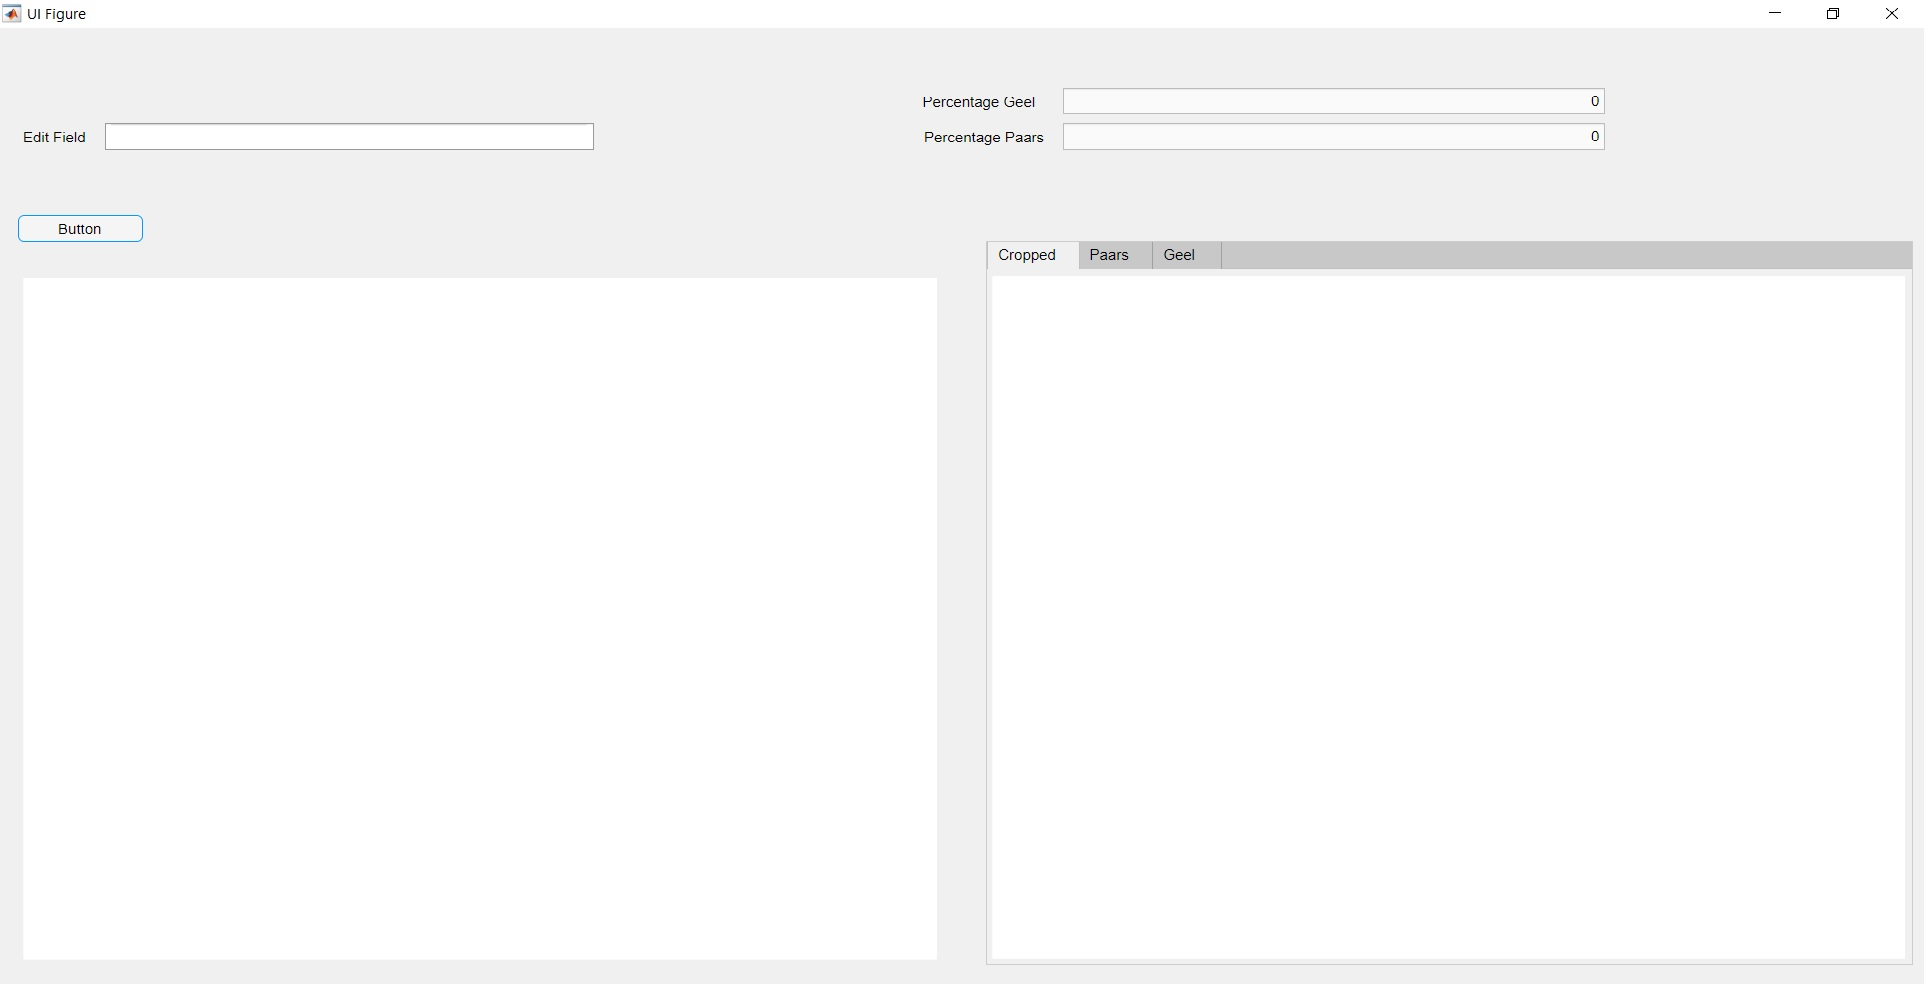
\includegraphics[width=170mm]{app.jpg}
			\caption{Voorstelling van de app}
			\label{fig: app}
		\end{figure}
	
		
	

	\section{Voorlopige resultaten}		
		Op dit moment kunnen we al effectief de foto gebruiksklaar maken voor de analyse ervan. Dit houdt in dat we alle pixels die niet tot de bloedklonter behoren wit kunnen maken en de afbeelding zodanig kunnen bijsnijden dat er geen overbodig geheugen ingenomen wordt door de afbeelding. In Figuur \ref{fig: voorna} wordt dit geïllustreerd.
	
		\begin{figure}[H]
			\centering
			\subfloat[Afbeelding van bloedklonter voor die bewerkt wordt]{{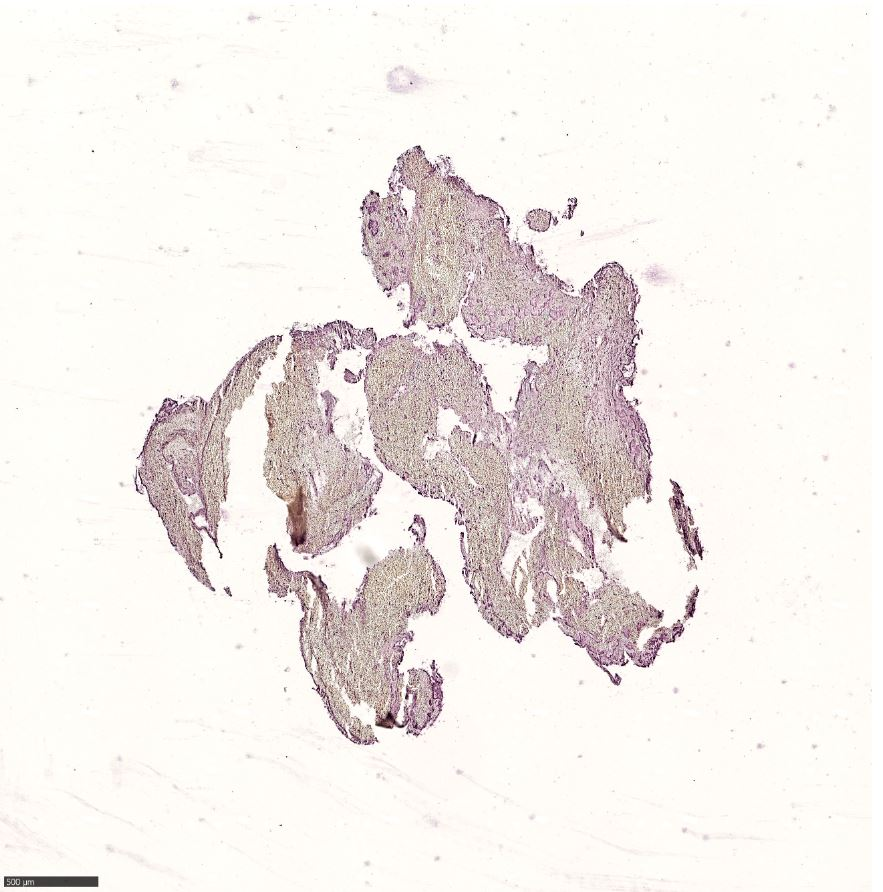
\includegraphics[width=4.5cm]{BloedklonterVoor.jpg}}}
			\qquad
			\subfloat[Bijgesneden afbeelding van de Bloedklonter met witte achtergrond ]{{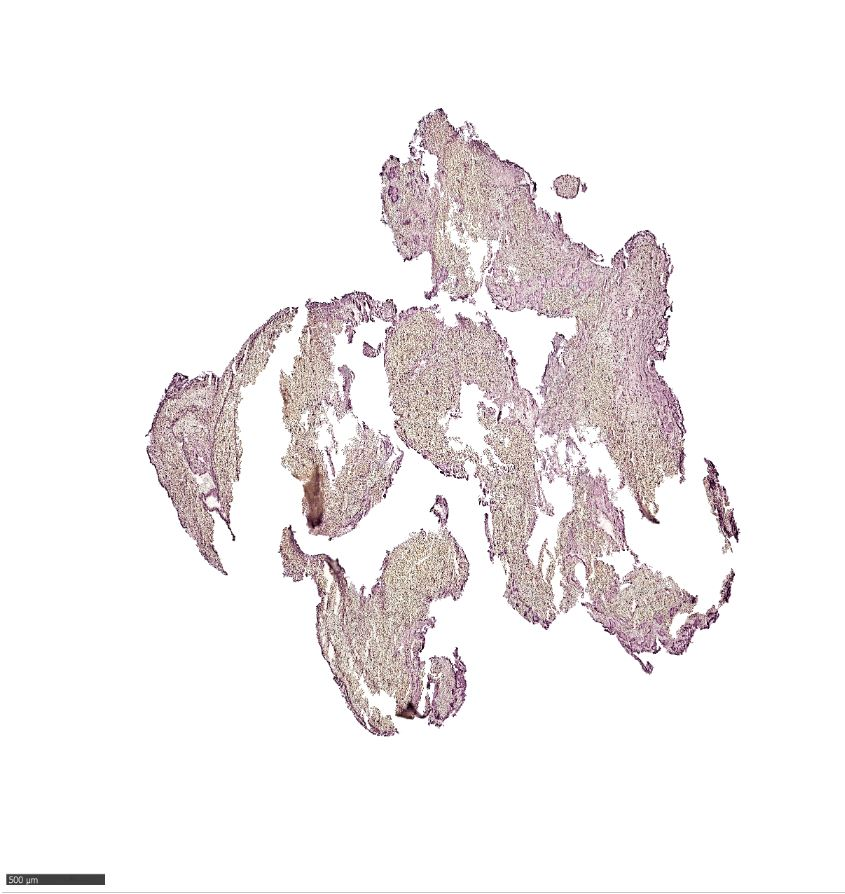
\includegraphics[width=4.5cm]{BloedklonterNa.jpg}}}
		
			\caption{Illustratie van hoe we de afbeelding gebruiksklaar maken voor de analyse ervan}
			\label{fig: voorna}
		\end{figure}
	
		Momenteel zijn we bezig met de implementatie van de kleurendetectie. We hebben hier al veel vooruitgang geboekt, maar de hij staat nog niet volledig op punt. Ook hebben we al even geëxperimenteerd met de app designer van Matlab. Hier willen we namelijk onze gebruiksvriendelijke applicatie in maken.
	
		Op basis van wat we nu al bereikt hebben, denken we dat dit project een succes kan worden en dat men het effectief zal kunnen gebruiken in het onderzoek naar de samenstelling van bloedklonters.
	
	\section{Verantwoordelijkheden en taakverdeling}		
		In onze groep hebben we ervoor gekozen om Robin aan te stellen als projectleider. Hij verdeelt elke week de taken en heeft het laatste woord bij discussies. 
		Voor de verslagen en de eindpresentatie is Marthe verantwoordelijk. Zij is de eindredactrice van alle verslagen. We schrijven de verslagen uiteraard samen, maar het is haar taak ervoor te zorgen dat deze volledig en gestructureerd zijn en dat ze voor de deadline ingediend worden. 
	
		Voor de implementatie van de code zijn we elk verantwoordelijk voor ons eigen deel. Zo wordt het verwijderen van de ruis en het bijsnijden van de afbeelding door Toon geleid, de kleurdetectie door Robin en de implementatie van de app door Marthe.
		
	\section{Integratie met vakken uit eerste 3 semsters}
		Om dit probleem op te lossen hebben we gebruik gemaakt van matlab. Het is dan ook een meerwaarde dat we in het eerste semester 'beginselen van programmeren' gehad hebben waardoor we sneller vertrouwd geraken met deze programmeertaal. Daarnaast leren we in 'nummerieke wiskunde' ook werken met matlab. Statistische analyse gebruiken we voor het analyseren van de verschillende kleuren.
	
	\section*{Besluit}	
		Afsluitende tekst

\end{document}
